\documentclass[a4paper, 14pt]{article}
\usepackage{tocloft}

\usepackage{amsthm}
\newtheorem{theorem}{Теорема}
\newtheorem{lemma}{Лемма}

\usepackage{setspace}
%\полуторный интервал
\onehalfspacing

\usepackage{arxiv}

\usepackage[T2A]{fontenc}
\usepackage[utf8]{inputenc}
\usepackage[english, russian]{babel}
% \usepackage{cmap}
\usepackage{url}
\usepackage{booktabs}
\usepackage{nicefrac}
\usepackage{microtype}
\usepackage{lipsum}
\usepackage{graphicx}
\usepackage{subfig}
\usepackage[square,sort,comma,numbers]{natbib}
\usepackage{doi}
\usepackage{multicol}
\usepackage{multirow}
\usepackage{tabularx}
\usepackage{color,colortbl} % Раскраска таблицы
\definecolor{Gray}{gray}{0.9}

\usepackage{tikz}
\usetikzlibrary{matrix}

% Algorithms
\usepackage{algpseudocode}
\usepackage{algorithm}

%% Шрифты
\usepackage{euscript} % Шрифт Евклид
\usepackage{mathrsfs} % Красивый матшрифт
\usepackage{extsizes} % Возможность сделать 14-й шрифт

\usepackage{makecell} % diaghead in a table
\usepackage{amsmath,amsfonts,amssymb,amsthm,mathtools,dsfont}
\usepackage{icomma}

\newcommand{\bz}{\mathbf{z}}
\newcommand{\bx}{\mathbf{x}}
\newcommand{\by}{\mathbf{y}}
\newcommand{\bv}{\mathbf{v}}
\newcommand{\bw}{\mathbf{w}}
\newcommand{\ba}{\mathbf{a}}
\newcommand{\bb}{\mathbf{b}}
\newcommand{\bp}{\mathbf{p}}
\newcommand{\bq}{\mathbf{q}}
\newcommand{\bt}{\mathbf{t}}
\newcommand{\bu}{\mathbf{u}}
\newcommand{\bs}{\mathbf{s}}
\newcommand{\bT}{\mathbf{T}}
\newcommand{\bX}{\mathbf{X}}
\newcommand{\bZ}{\mathbf{Z}}
\newcommand{\bS}{\mathbf{S}}
\newcommand{\bH}{\mathbf{H}}
\newcommand{\bW}{\mathbf{W}}
\newcommand{\bY}{\mathbf{Y}}
\newcommand{\bU}{\mathbf{U}}
\newcommand{\bQ}{\mathbf{Q}}
\newcommand{\bP}{\mathbf{P}}
\newcommand{\bA}{\mathbf{A}}
\newcommand{\bB}{\mathbf{B}}
\newcommand{\bC}{\mathbf{C}}
\newcommand{\bE}{\mathbf{E}}
\newcommand{\bF}{\mathbf{F}}
\newcommand{\bomega}{\boldsymbol{\omega}}
\newcommand{\btheta}{\boldsymbol{\theta}}
\newcommand{\bgamma}{\boldsymbol{\gamma}}
\newcommand{\bdelta}{\boldsymbol{\delta}}
\newcommand{\bPsi}{\boldsymbol{\Psi}}
\newcommand{\bpsi}{\boldsymbol{\psi}}
\newcommand{\bxi}{\boldsymbol{\xi}}
\newcommand{\bchi}{\boldsymbol{\chi}}
\newcommand{\bzeta}{\boldsymbol{\zeta}}
\newcommand{\blambda}{\boldsymbol{\lambda}}
\newcommand{\beps}{\boldsymbol{\varepsilon}}
\newcommand{\bZeta}{\boldsymbol{Z}}
% mathcal
\newcommand{\cX}{\mathcal{X}}
\newcommand{\cY}{\mathcal{Y}}
\newcommand{\cW}{\mathcal{W}}

\newcommand{\dH}{\mathds{H}}
\newcommand{\dR}{\mathds{R}}
% transpose
\newcommand{\T}{^{\mathsf{T}}}

% \renewcommand{\shorttitle}{\textit{arXiv} Шаблон}
\renewcommand{\epsilon}{\ensuremath{\varepsilon}}
\renewcommand{\phi}{\ensuremath{\varphi}}
\renewcommand{\kappa}{\ensuremath{\varkappa}}
\renewcommand{\le}{\ensuremath{\leqslant}}
\renewcommand{\leq}{\ensuremath{\leqslant}}
\renewcommand{\ge}{\ensuremath{\geqslant}}
\renewcommand{\geq}{\ensuremath{\geqslant}}
\renewcommand{\emptyset}{\varnothing}

\usepackage{hyperref}
% \usepackage[usenames,dvipsnames,svgnames,table,rgb]{xcolor}

\hypersetup{
	unicode=true,
	pdftitle={A template for the arxiv style},
	pdfsubject={q-bio.NC, q-bio.QM},
	pdfauthor={David S.~Hippocampus, Elias D.~Striatum},
	pdfkeywords={First keyword, Second keyword, More},
	colorlinks=true,
	linkcolor=black,        % внутренние ссылки
	citecolor=blue,         % на библиографию
	filecolor=magenta,      % на файлы
	urlcolor=blue           % на URL
}

\graphicspath{{../figures/}}

\usepackage{enumitem} % Для модификаций перечневых окружений

\theoremstyle{definition} % "Определение"
\newtheorem{definition}{Опр.}[section]

\usepackage{etoolbox}

\makeatletter
\expandafter\patchcmd\csname\string\algorithmic\endcsname{\itemsep\z@}{\itemsep=1.5mm}{}{}
\makeatother
%%% Титульный лист
% \thispagestyle{empty}

\begin{titlepage}
    \begin{center}
        \textsc{Московский физико-технический институт}\\
        (национальный исследовательский университет)\\
        \textsc{Физтех-школа прикладной математики и информатики}\\
        \textsc{Кафедра интеллектуальных систем}
        \end{center}
        \vspace{1.5cm}
        \begin{center}
        {Никитина Мария Александровна}
        \par
        \vspace{2cm}
        {\Large \textsc{\textbf{Анализ смещения распределений при использовании сравнительного подхода в обучении представлений данных}}}
        \par
        \vspace{2cm}
        {03.03.01~--- Прикладные математика и физика}
        \par
        \vspace{1.5cm}
        \textsc{Выпускная квалификационная работа бакалавра}
        \end{center}
        \vspace{1.5cm}
        \hfill\parbox{8,4cm}{\textbf{Научный руководитель:}
        \\к.ф.-м.н. Р.\,В.\,Исаченко}
        \par
        \vspace{2.5cm}
        \begin{center}
        {Москва~--- 2024}
    \end{center}
\end{titlepage}
% \setcounter{page}{2}

\renewcommand{\abstractname}{Аннотация}

\title{Анализ смещения распределений при использовании сравнительного подхода в обучении представлений данных}

\author{
    Мария Никитина \\
	\texttt{nikitina.mariia@phystech.edu} \\
	\And
 	Роман Исаченко \\
	\texttt{roman.isachenko@phystech.edu}
}
\date{\today}

\usepackage{setspace}
%\полуторный интервал
\onehalfspacing

\begin{document}
% \maketitle
% \thispagestyle{empty}

\begin{titlepage}
    \begin{center}
        \textsc{Московский физико-технический институт}\\
        (национальный исследовательский университет)\\
        \textsc{Физтех-школа прикладной математики и информатики}\\
        \textsc{Кафедра интеллектуальных систем}
        \end{center}
        \vspace{1.5cm}
        \begin{center}
        {Никитина Мария Александровна}
        \par
        \vspace{2cm}
        {\Large \textsc{\textbf{Анализ смещения распределений при использовании сравнительного подхода в обучении представлений данных}}}
        \par
        \vspace{2cm}
        {03.03.01~--- Прикладные математика и физика}
        \par
        \vspace{1.5cm}
        \textsc{Выпускная квалификационная работа бакалавра}
        \end{center}
        \vspace{1.5cm}
        \hfill\parbox{8,4cm}{\textbf{Научный руководитель:}
        \\к.ф.-м.н. Р.\,В.\,Исаченко}
        \par
        \vspace{2.5cm}
        \begin{center}
        {Москва~--- 2024}
    \end{center}
\end{titlepage}
\setcounter{page}{2}

\begin{abstract}
Контрастное обучение -- распространённый подход в сфере обучения без учителя. Данный метод заключается в попарном сравнении представлений объектов выборки для восстановления распределения в пространстве представлений. При этом похожие представления находятся близко, а отличающиеся -- далеко. Однако исходное распределение и способ порождения данных неизвестны, а функции потерь имеют несколько локальных минимумов, не все из которых соответствуют истинному распределению. В данной работе в качестве решения данных проблем приводятся функции потерь, устраняющие смещение распределений вследствие наличия ложноотрицательных и ложноположительных пар в разметке. Предлагается несмещённая модель контрастного обучения, исследуются её свойства. Качество полученного представления оценивается  в задаче классификации и в задаче VQA, для которых предложенная модель показала результат лучше, чем модель, не учитывающая смещение. Также проводится эксперимент на искусственной выборке из двумерного пространства, в котором проверяется качество восстановления исходного распределения предложенной моделью.
\end{abstract}

\keywords{Contrastive learning \and Representation learning \and Self-supervised learning}

\newpage
% \pagenumbering{roman} % use lowercase Roman numerals for page numbering before the main content

\tableofcontents
\clearpage % start the table of contents on a new page

% \pagenumbering{arabic}

\section{Введение}

Методы обучения без учителя не требуют предварительной разметки данных, а, значит, для них легче найти большие по объёму выборки для предобучения универсальной модели, которая далее на небольшом датасете подстраивается под требуемую задачу.

\textit{Самообучение} -- класс методов, позволяющих модели обучаться на датасетах без явной разметки. Вместо этого используются некоторые наблюдаемые характеристики выборки.

В частности, \textit{обучение представлениям} -- это процесс отображения необработанных входных данных в пространство векоторов-признаков или тензоров с целью найти и извлечь полезные закономерности, которые будут полезны для предсказания целевых значений.

Первые модели машинного обучения использовались для принятия решений на основе извлеченных с помощью предобработки признаков. Увеличение объема доступных вычислений и размеченных датасетов позволило перейти от использования средств извлечения признаков, разработанных вручную, к моделям, автоматически выделяющим особенности выборки. В результате исследования также сместились с разработки признаков на разработку архитектуры модели, которая самостоятельно может создавать представление данных.

Задача поиска хорошего представления достаточно сложная. Согласно \citep{LeKhac2020}, существует несколько принципов, на которых строится обучение представлениям: выразительность и способность кодировать экспоненциальное число конфигураций в отличие от методов наподобие one-hot, абстрактность и отсутствие сильной зависимости от локальных возмущений, непротиворечивость и обеспечение наглядности представления. Одно из решений -- \textit{контрастное обучение или обучение сравнениями} -- подход, при котором обучение происходит не только по принципу близости, но и по принципу различия. В отличие от дискриминативной модели, которая учится моделировать границу принятия решений среди классов, и генеративной модели, которая реконструирует распределение входной выборки, при констрастном обучении представление изучается путем сравнения пар элементов \citep{Chopra}. Пусть вектор $\textbf{x}$ некоторого объекта принят за основной. Тогда вектор схожего объекта $\textbf{x}^+$ -- положительный элемент. Он должен располагаться как можно ближе к $\textbf{x}$ в пространстве эмбеддингов ввиду гипотезы о генерации данных из распределения, в котором расстояние между схожими элементами минимально. А вектор отличного объекта $\textbf{x}^-$ -- как можно дальше, как негативный элемент. Основной сложностью использования такого подхода является правильный подбор негативных и позитивных элементов при отсутствии разметки в данных.

Одни из распространённых мер различия элементов: \textit{Triplet loss} \citep{Schroff2015} и его модификация для $N$ негативных примеров -- \textit{мультиклассовый N-pair loss} \citep{Sohn2016ImprovedDM}, а также \textit{Information Noise-Contrastive Estimation} или \textit{InfoNCE} \citep{NCE}, \citep{Oord2018RepresentationLW} как обобщение N-pair loss.

Triplet loss был впервые использован в задаче распознавания одного и того же человека в разных позах и под разным углом. Пусть есть элемент $\mathbf{x}$. Один положительный элемент $\textbf{x}^+$ и один отрицательный $\textbf{x}^-$ выбираются с предположением, что $\textbf{x}^+$ принадлежит к тому же классу, что и $\mathbf{x}$, а $\mathbf{x}^-$ -- к другому. Обучение модели направлено на уменьшение расстояния между эмбеддингами $\mathbf{x}$ и $\mathbf{x}^+$ и увеличение расстояния между эмбеддингами $\mathbf{x}$ и $\mathbf{x}^-$:

\begin{equation}
    \mathcal{L}_{Triplet}(\textbf{x}, \textbf{x}^+, \{\textbf{x}_i^-\}) = \sum\limits_{x \in \chi}\max(0, ||f(\textbf{x}) - f(\textbf{x}^+)||_2^2 - ||f(\textbf{x}) - f(\textbf{x}^-)||_2^2 + \epsilon.
\end{equation}

В задачах распознавания изображений распространённым методом выбора положительной пары является аугментация основного изображения, а в качестве отрицательных пар берутся все остальные $N - 1$ элементов в батче. Для случая $N - 1$ негативных векторов существует обобщение $\mathcal{L}_{Triplet}(\textbf{x}, \textbf{x}^+, \{\textbf{x}_i^-\})$:

\begin{equation}\label{eq:103}
    \mathcal{L}_{N-pair}(\textbf{x}, \textbf{x}^+, \{\textbf{x}_i^-\}_{i=1}^{N-1}) = - \log \frac{\exp(f(\textbf{x})^T f(\textbf{x}_i^+))}{\exp(f(\textbf{x})^T f(\textbf{x}_i^+)) + \sum _{i=1}^{N-1} \exp(f(\textbf{x})^Tf(\textbf{x}_i^-))}.
\end{equation}

Если вместо $\exp(f(\textbf{x})^T f(\textbf{c}))$ брать любую функцию, аппроксимирующую $\frac{p(\textbf{x}|\textbf{c})}{p(\textbf{x})}$, получится InfoNCE loss:

\[\mathcal{L}_{InfoNCE} = -\mathbb{E}\left[\log\frac{f(\textbf{x}, \textbf{c})}{\sum_{\mathbf{x}' \in X}f(\textbf{x}', \textbf{c})}\right].\]

Методы обучения сравнениями имеют хороший результат в формировании визуальных представлений. Например, в \citep{chen2020simple} представлен фреймворк SimCLR, значительно превосходящий предыдущие методы самообучения. Его авторы разработали NT-Xent, в котором используется косинусное расстояние вместо скалярных произведений:

\[\mathcal{L}_{SimCLR}^{(i, j)} = - \log\frac{\exp(\text{sim}(g(\mathbf{h}_i), g(\mathbf{h}_j)) / \tau)}{\sum\limits_{i \neq k}^{2N}\exp(\text{sim}(g(\mathbf{h}_i), g(\mathbf{h}_k)) / \tau)},\]

\noindent где $\mathbf{h}_i = f(\mathbf{x})$, то есть вместо вектора из сформированного пространства представлений в функцию потерь входит его проекция на некоторое другое пространство. Также в \citep{zbontar2021barlow} представлена идея сравнения эмбеддингов с помощью кросс-корреляции.

В методах самообучения отсутствие истинных меток приводит к необходимости случайного выбора отрицательных экземпляров $\mathbf{x}^-$. Однако такой подход приводит к смещению, если $\mathbf{x}^-$ на самом деле достаточно похож на $\mathbf{x}$, например, фотографии одного и того же объекта с разных ракурсов. В таком случае смещение приводит к отдалению близких элементов в пространстве эмбеддингов и, как следствие, к значительному снижению качества \citep{NEURIPS2021_de8aa43e}.

В \citep{chuang2020debiased} предложена несмещённая контрастная функция потерь. Учитывается $N$ отрицательных и $M$ положительных элементов из выборки. $L^{N, M}_{\text{Neg}}(f)$ -- функция потерь, корректирующая смещение ввиду наличия ложноотрицательных экземпляров. Чтобы избавиться от необходимости разметки, элементы берутся из распределения данных, а положительное распределение создаётся искусственно с помощью аугментаций, которые могут содержать ложноположительные выбросы.

Эта работа направлена на разработку нового алгоритма для снижения вероятности смещения при появлении ложноположительных и ложноотрицательные элементов, а также оценку качества восстановления исходного распределения данных в пространстве эмбеддингов.

\newpage
\section{Предыдущие исследования}
Основная задача данного исследования -- создание функции потерь, учитывающей смещение в данных и анализ её способности восстанавливать исходное распределение, из которого были порождены данные, в пространстве эмбеддинов. Идея учёта смещения в функции потерь путём введения скрытых классов и вероятностей получить для элементов $\textbf{x}$ и $\textbf{x}^+$ один и тот же класс описана в \citep{chuang2020debiased} и \citep{Arora2019ATA}. В качестве распределения в скрытом пространстве берётся равномерное в предположении, что темы в лучшем пространстве эмбеддингов должны быть распределены подобным образом. Одна из рассматриваемых задач -- классификация на неразмеченных данных. В этом случае большое влияние на качество результата оказывает подбор для $\textbf{x}$ отрицательных пар. Ввиду того, что в качестве положительных пар берутся различные аугментации данного изображения, а в качестве отрицательных -- все остальные картинки в батче, появляется вероятность получить ложноотрицательные пары, так как есть вероятность, что не все изображения в выборке имеют класс, отличный от класса элемента $\textbf{x}$. В \citep{chuang2020debiased} в функции потерь вероятность получить отрицательную пару выражается через полную вероятность и вероятность получить положительную пару. Тем самым приближается неизвестное распределение отрицательных элементов в выборке.

В \citep{ALBEF} и \citep{TCL} рассматривается применение обучения сравнениями в задаче сопоставления картинок и текстов для предобучения. В \citep{ALBEF} InfoNCE loss используется не только для сопоставления похожих картинок к картинкам, а текстов к текстам, но и для приближения эмбеддингов близких по смыслу картинок и текстов в одном пространстве перед тем, как передать их мультимодальной модели. Однако в \citep{TCL}, в отличие от \citep{ALBEF}, также учитывается проблема того, что обычно в изображении хранится больше информации, чем описано в тексте. В \citep{TCL} применяется локальное выравнивание для максимизации совместной информации между локальным и глобальным представлениями. Итоговая функция потерь в данном фреймворке состоит из кросс-модального выравнивания, где InfoNCE loss применяется для сравнения картинки с текстом и текста с картинкой:

\begin{equation}
    \mathcal{L}_{nce}(\mathbf{I}, \mathbf{T}_+, \{\mathbf{T}_k\}_{k=1}^K) = - \mathbb{E}_{p(\mathbf{I}, \mathbf{T})}\left[\log\frac{e^{(\text{sim}(\mathbf{I}, \mathbf{T}_+)/\tau)}}{\sum_{k=1}^Ke^{(\text{sim}(\mathbf{I}, \mathbf{T}_k)/\tau)}}\right],
\end{equation}

\noindent где $\tau$ -- параметр температуры, $\mathbf{T}_+$ -- положительный текстовый семпл, $\{\mathbf{T}_k\}_{k=1}^K$ -- множество негативных текстовых семплов, $\text{sim}(\mathbf{I}, \mathbf{T}_k) = f_\mathbf{v}(\mathbf{v})^\top \hat{f}_\mathbf{t}(\hat{\mathbf{t}})$, где $f_\mathbf{v}$ и $\hat{f}_\mathbf{t}$ -- проекции выходов визуального и текстового энкодеров на пространство, в котором применяется функция потерь. Для выбора отрицательных текстовых элементов используется идея, берущая начало с \textit{банка памяти} из \citep{MemoryBank}, который для уменьшения числа вычислений эмбеддингов хранит представления с предыдущих итераций, что увеличивает затраты по памяти, но значительно уменьшает время работы модели. Эта идея имеет развитие в \citep{he2019moco}, где используются эмбеддинги не самой модели, а её версии с моментумом для избавления от шума, являющегося большой проблемой для больших датасетов, собранных без разметки из интернета. Таким образом, $\hat{\mathbf{t}}$ -- эмбеддинг, полученный с помощью модели с моментумом, а $\hat{f}_\mathbf{t}$ -- функция, действующая на пространстве таких представлений. То есть параметры модели, вычисляющей хранимые эмбеддинги, представляют собой скользящее среднее по эпохам. Использование сети со скользящим средним имеет развитие в \citep{grill2020bootstrap}, где не требуется сэмплирование отрицательных элементов.

Аналогично определяется вторая часть данной функции потерь, высчитываемая относительно текста, а не изображения:

\begin{equation}
    \mathcal{L}_{nce}(\mathbf{T}, \mathbf{I}_+, \{\mathbf{I}_k\}_{k=1}^K) = - \mathbb{E}_{p(\mathbf{I}, \mathbf{T})}\left[\log\frac{e^{(\text{sim}(\mathbf{T}, \mathbf{I})/\tau)}}{\sum_{k=1}^Ke^{(\text{sim}(\mathbf{T}, \mathbf{I}_k)/\tau)}}\right],
\end{equation}

\begin{equation}\label{eq:cma}
    \mathcal{L}_{cma} = \frac{1}{2}[\mathcal{L}_{nce}(\mathbf{I}, \mathbf{T}_+, \{\mathbf{T}_k\}_{k=1}^K) + \mathcal{L}_{nce}(\mathbf{T}, \mathbf{I}_+, \{\mathbf{I}_k\}_{k=1}^K)].
\end{equation}

Помимо кросс-модального сравнения, итоговая функция потерь включает в себя внутримодальное выравнивание, где InfoNCE loss применяется для сравнения картинки с картинкой и текста с текстом. Такое выравнивание используется, так как объекты разной модальности зачастую не могут полностью описать друг друга. В таком случае необходимо выравнивание ещё и внутри каждой модальности, чтобы приблизить друг к другу различные аугментации одно и того же элемента данных:

\begin{equation}\label{eq:imc}
    \mathcal{L}_{imc} = \frac{1}{2}[\mathcal{L}_{nce}(\mathbf{T}, \mathbf{T}_+, \{\mathbf{T}_k\}_{k=1}^K) + \mathcal{L}_{nce}(\mathbf{I}, \mathbf{I}_+, \{\mathbf{I}_k\}_{k=1}^K)].
\end{equation}

Для того чтобы учитывать не только глобальную информацию с изображений и текста, но и локальную, в итоговую функцию потерь в \citep{TCL} добавляется локальная максимизация, в которой с помощью InfoNCE loss часть изображения сравнивается со всем изображением, а часть текста -- со всем текстом:

\begin{equation}\label{eq:lmi}
    \mathcal{L}_{lmi} = \frac{1}{2}\left[\frac{1}{M}\sum\limits_{i=1}^M\mathcal{L}_{nce}(\mathbf{T}, \mathbf{T}_+^i, \{\mathbf{T}_k\}_{k=1}^K) + \frac{1}{N}\sum\limits_{j=1}^N\mathcal{L}_{nce}(\mathbf{I}, \mathbf{I}_+^j, \{\mathbf{I}_k\}_{k=1}^K)\right],
\end{equation}

\noindent где $\mathbf{T}^i$ -- $i$-ая часть изображения, $\mathbf{I}^j$ -- $j$-ая часть текста.

Для соединения представления картинок и текстов используется задача бинарной классификации предсказания, положительна пара или отрицательна, где в качестве таргета используется результат применения функции потерь из кросс-модального выравнивания, а в качестве предсказания -- выход полносвязного слоя мультимодального энкодера:

\begin{equation}
    \mathcal{L}_{itm} = \mathbb{E}_{p(\mathbf{I}, \mathbf{T})}H(\phi(\mathbf{I}, \mathbf{T}), y^{(\mathbf{I}, \mathbf{T})}),
\end{equation}

\noindent где $H(;)$ -- кросс-энтропия, $y^{(\mathbf{I}, \mathbf{T})}$ -- таргет.

Маскированная текстовая модель, в которой слова с вероятностью 15\% заменяются на специальный токен [MASK] или случайное слово, используется для того, чтобы снизить влияние шума, распространённого для больших датасетов, и улучшения гибкости модели в использовании синонимов. Предсказание пропущенного слова основывается на контексте текста и изображения:

\begin{equation}
    \mathcal{L}_{mlm} = \mathbb{E}_{p(\mathbf{I}, \mathbf{T}^{msk})}H(\Phi(\mathbf{I}, \mathbf{T}^{msk}), y^{\mathbf{T}^{msk}}),
\end{equation}

\noindent где $\Phi(\mathbf{I}, \mathbf{T}^{msk})$ -- предсказанная вероятность $\mathbf{T}^{msk}$, $y^{\mathbf{T}^{msk}}$ -- настоящий токен.

Итоговая функция потерь в \citep{TCL}:

\begin{equation}
    \mathcal{L} = \mathcal{L}_{cma} + \mathcal{L}_{imc} + \mathcal{L}_{lmi} + \mathcal{L}_{itm} + \mathcal{L}_{mlm}.
\end{equation}

Обоснование применения InfoNCE заключается в том, что он связан с нижней границей совместной информации, которую тяжело посчитать напрямую. Уменьшение InfoNCE увеличивает взаимную информацию внутри положительной пары. В \citep{Oord2018RepresentationLW} представлено доказательство, использующее связь функции потерь с MINE \citep{belghazi2021mine}.

\newpage
\section{Постановка задачи}

\subsection{Несмещённая функция потерь}

Пусть $\mathcal{X}$ -- предметное пространство. Обучение сравнениями работает с семантически близкими парами точек $(\mathbf{x}, \mathbf{x}^+)$, где $\mathbf{x}$ берётся из распределения данных $p(\mathbf{x})$ над $\mathcal{X}$. Цель состоит в том, чтобы найти функцию эмбеддинга $f: \mathcal{X} \rightarrow \mathbb{R}^d$. В \citep{chuang2020debiased} предполагается, что существует множество дискретных скрытых классов $\mathcal{C}$ и положительные пары $(\mathbf{x}, \mathbf{x}^+)$ имеют один и тот же класс. Распределение по $\mathcal{C}$ обозначается $\rho(c)$, следовательно, совместное распределение $p_{\mathbf{x},c}(\textbf{x}, c) = p(\textbf{x}|c)\rho(c)$. Пусть $h : \mathcal{X} \rightarrow \mathcal{C}$ -- функция, присваивающая метки классов. Тогда $p^+_\mathbf{x}(\textbf{x}') = p(\textbf{x}'|h(\textbf{x}') = h(\textbf{x}))$ -- вероятность сказать, что $\textbf{x}'$ -- положительная пара для $\textbf{x}$, и $p^-_\mathbf{x}(\textbf{x}') = p(\textbf{x}'|h(\textbf{x}') \neq h(\textbf{x}))$ -- для отрицательной пары. Предполагается, что вероятности классов $\rho(\textbf{x}^+) = \tau^+$ однородны и $\tau^- = 1 - \tau^+$ -- вероятность обнаружить любой другой класс. Тогда «идеальный» N-pair loss при условии наличия $N$ негативных элементов выглядит так:

\begin{equation}\label{eq:1}
\mathcal{L}_{\text{Unbiased}}^N(f) = \mathbb{E}_{\substack{\textbf{x} \sim p_\mathbf{x}, \textbf{x}^+ \sim p^+_\mathbf{x},\\ \textbf{x}_i^- \sim p_\mathbf{x}^-}} \bigg[-\log \frac{e^{f(\textbf{x})^T f(\textbf{x}^+)}}{e^{f(\textbf{x})^T f(\textbf{x}^+)} + \sum _{i=1}^N e^{f(\textbf{x})^T f(\textbf{x}_i^-)}}\bigg].
\end{equation}

На практике $p_\mathbf{x}^-(\textbf{x}_i^-)$ неизвестно, поэтому $\textbf{x}_i^-$ выбирается из немаркированного распределения $p(\textbf{x})$. $\tau^+$ -- вероятность появления ложноотрицательного элемента. Функция потерь для такого случая уже будет смещённой.

\begin{equation}\label{eq:2}
\mathcal{L}_{\text{Biased}}^N(f) = \mathbb{E}_{\substack{\textbf{x} \sim p_\mathbf{x}, \textbf{x}^+ \sim p^+_\mathbf{x},\\ \textbf{x}_i^- \sim p_\mathbf{x}}} \bigg[-\log \frac{e^{f(\textbf{x})^T f(\textbf{x}^+)}}{e^{f(\textbf{x})^T f(\textbf{x}^+)} + \sum _{i=1}^N e^{f(\textbf{x})^T f(\textbf{x}_i^-)}}\bigg].
\end{equation}

Доказательство леммы о том, что в пределе при $N \to \infty$ функция потерь $L_{\text{Biased}}^N(f)$ является верхней гранью $L_{\text{Unbiased}}^N(f)$, представлено в \citep{chuang2020debiased}.

Распределение $p(\mathbf{x})$ при условии наличия $M$ положительных элементов можно разложить:

\begin{equation}\label{eq:3}
p(\textbf{x}') = \tau^+ p^+_\mathbf{x}(\textbf{x}') + \tau^-p_\mathbf{x}^-(\textbf{x}').
\end{equation}

Выразим $p^-_\mathbf{x}(\textbf{x}')$:

\begin{equation} \label{eq:4}
p_\mathbf{x}^-(\textbf{x}') = \frac{p(\textbf{x}') - \tau^+ p^+_\mathbf{x}(\textbf{x}')}{\tau^-}.
\end{equation}

Подсчёт $p^-_x(\textbf{x}')$ через $p(\mathbf{x})$ и $p^+_x(\textbf{x}')$ в итоговой формуле достаточно дорогостоящий. Поэтому в \citep{chuang2020debiased} предлагается использовать приближение итоговой функции потерь:

\begin{equation}\label{eq:5}
\mathcal{L}_{\text{Neg}}^{N, M}(f) = \mathbb{E}_{\substack{\textbf{x} \sim p; \textbf{x}_+ \sim p_\mathbf{x}^+,\\ \{\textbf{u}_i\}_{i=1}^N \sim p^N \\ \{\textbf{v}_j\}_{j=1}^M \sim {p_\mathbf{x}^+}^M}}  \bigg[ -\log \frac{e^{f(\textbf{x})^T f(\textbf{x}^+)} }{e^{f(\textbf{x})^T f(\textbf{x}^+)} + N g\big(\textbf{x}, \{\textbf{u}_i\}_{i=1}^N, \{\textbf{v}_j\}_{j=1}^M\big)} \bigg],
\end{equation}

\noindent где эмпирическая оценка $p(\mathbf{x}^-)$:

\begin{equation}\label{eq:6}
g\big(\textbf{x}, \{\textbf{u}_i\}_{i=1}^N, \{\textbf{v}_j\}_{j=1}^M\big) = \max \bigg\{ \frac{1}{\tau^-}\bigg(\frac{1}{N} \sum \limits_{i=1}^N e^{f(\textbf{x})^T f(\textbf{u}_i)} - \tau^+ \frac{1}{M} \sum \limits_{j=1}^M e^{f(\textbf{x})^T f(\textbf{v}_j)}\bigg), e^{-1/t}\bigg\},
\end{equation}

\noindent где $\{\textbf{u}_i\}_{i=1}^N$ -- $N$ сэмплов из $p(\mathbf{x'})$ и $\{\textbf{v}_j\}_{j=1}^M$ -- $M$ сэмплов из $p(\mathbf{x'}^+)$, $t$ -- параметр температуры.

% В \citep{chuang2020debiased} также приводится оценка скорости сходимости $L_{\text{Neg}}^{N, M}(f)$ к случаю бесконечного $N$ и $M = 1$:

% \begin{equation}\label{eq:102}
% |\tilde{L}_{\text{DebiasedNeg}}^N(f) - L_{\text{DebiasedNeg}}^{N, M}(f)| \leq \frac{e^{3/2}}{\tau^-}\sqrt{\frac{\pi}{2N}} + \frac{e^{3/2}\tau^+}{\tau^-}\sqrt{\frac{\pi}{2M}}
% \end{equation}

Применение данной функции потерь в модели SimCLR позволило смоделировать смещение при наличии в выборке ложноотрицательных элементов и увеличить точность результата. В данной работе будет произведено её сравнение с функцией потерь, в которой вместо $p(\mathbf{x}^-)$ будет выражен $p(\mathbf{x}^+)$.

\subsection{Ложноположительные элементы}

Чрезмерная аугментация делает положительную пару достаточно далёкой в начальном пространстве и приводит к появлению ложноположительных объектов и смещению оценки. При недостатке вычислительных ресурсов при аугментации некоторая часть из изображения вырезается. Оставшаяся часть может сильно отличаться от второй аугментации. Чем меньше размер вырезанного изображения, тем больше вероятность появления ложноположительной пары. Распределение положительных элементов в рамках функции потерь представляется таким образом:

\begin{equation}\label{eq:7}
p_\mathbf{x}^+ (\textbf{x}') = \frac{p(\textbf{x}') - \tau^- p^-_\mathbf{x}(\textbf{x}')}{\tau^+}.
\end{equation}

\begin{lemma}
\label{lemm:asympt}
% \normalfont 
При $N \to \infty$ несмещённая функция потерь стремится к функции потерь, учитывающей наличие ложноположительных элементов:
\begin{equation} \label{eq:8}
\begin{split}
\mathcal{L}_{\text{Unbiased}}^N(f) = \mathbb{E}_{\substack{\mathbf{x} \sim p \\ \mathbf{x}^+ \sim p_\mathbf{x}^+ \\ \{\mathbf{x}_i^-\}_{i=1}^N \sim {p_\mathbf{x}^-}^N}} \bigg[ - \log \frac{e^{f(\mathbf{x})^T f(\mathbf{x}^+)}}{e^{f(\mathbf{x})^T f(\mathbf{x}^+)} + \sum_{i=1}^N e^{f(\mathbf{x})^T f(\mathbf{x}_i^-)}} \bigg] \longrightarrow \\
\longrightarrow \mathbb{E}_{\substack{\mathbf{x} \sim p \\ \mathbf{x}^- \sim p_\mathbf{x}^-}} \bigg[ - \log \frac{R}{R + N \mathbb{E}_{\mathbf{x}^- \sim p_\mathbf{x}^-} e^{f(\mathbf{x})^T f(\mathbf{x}^-)}} \bigg],
\end{split}
\end{equation}

\noindent где
\begin{equation}\label{eq:9}
R = \frac{1}{\tau^+} \big(\mathbb{E}_{\mathbf{x}' \sim p} e^{f(\mathbf{x})^T f(\mathbf{x}')} - \tau^- \mathbb{E}_{\mathbf{x}^- \sim p_\mathbf{x}^-} e^{f(\mathbf{x})^T f(\mathbf{x}^-)}\big).
\end{equation}
\end{lemma}

\renewcommand\qedsymbol{$\blacksquare$}
\begin{proof}
Для того чтобы внести предел под знак математического ожидания, можно применить теорему Леви о монотонной сходимости. Для неё требуется, чтобы последовательность положительных измеримых функций под знаком математического ожидания была монотонно возрастающей. Тогда пусть $h_N(\mathbf{x}) = - \log \frac{e^{f(\textbf{x})^T f(\textbf{x}^+)}}{e^{f(\textbf{x})^T f(\textbf{x}^+)} + \sum_{i=1}^N e^{f(\textbf{x})^T f(\textbf{x}_i^-)}}$ -- измеримая, как композиция измеримых функций.

Так как ввиду положительности экспоненты

\[\frac{e^{f(\textbf{x})^T f(\textbf{x}^+)}}{e^{f(\textbf{x})^T f(\textbf{x}^+)} + \sum_{i=1}^N e^{f(\textbf{x})^T f(\textbf{x}_i^-)}} \leq 1,\]

\noindent то последовательность $\{h_N(\mathbf{x})\}_{N=1}^{\infty}$ состоит из положительных функций.

\[\frac{e^{f(\textbf{x})^T f(\textbf{x}^+)}}{e^{f(\textbf{x})^T f(\textbf{x}^+)} + \sum_{i=1}^N e^{f(\textbf{x})^T f(\textbf{x}_i^-)}} \geq \frac{e^{f(\textbf{x})^T f(\textbf{x}^+)}}{e^{f(\textbf{x})^T f(\textbf{x}^+)} + \sum_{i=1}^N e^{f(\textbf{x})^T f(\textbf{x}_i^-)} + e^{f(\textbf{x})^T f(\textbf{x}_{N+1}^-)}}.\]

Следовательно, так как логарифм -- монотонная функция, а в математическом ожидании он умножается на $-1$, последовательность $\{h_N(\mathbf{x})\}_{N=1}^{\infty}$ монотонно возрастает:

\[0 \leq h_N(\mathbf{x}) \leq h_{N+1}(\mathbf{x}).\]

Так как $h = - \log \frac{\mathbb{E}_{\textbf{x}^+ \sim p_\mathbf{x}^+} e^{f(\textbf{x})^T f(\textbf{x}^+)}}{\mathbb{E}_{\textbf{x}^+ \sim p_\mathbf{x}^+} e^{f(\textbf{x})^T f(\textbf{x}^+)} + N \mathbb{E}_{\textbf{x}^- \sim p_\mathbf{x}^-} e^{f(\textbf{x})^T f(\textbf{x}^-)}}$ -- измеримая функция, то, учитывая доказательство выше, можно утверждать, что условия теоремы Леви выполнены. Тогда:

\[\lim\limits_{N \to \infty} \mathbb{E} h_N(\mathbf{x}) = \mathbb{E} h(\mathbf{x}).\]

Переходя к исходным обозначениям:

\begin{equation}
\begin{split}
\lim_{N \to \infty} \mathbb{E} \bigg[ - \log \frac{e^{f(\textbf{x})^T f(\textbf{x}^+)}}{e^{f(\textbf{x})^T f(\textbf{x}^+)} + \sum_{i=1}^N e^{f(\textbf{x})^T f(\textbf{x}_i^-)}} \bigg] = \\
= \mathbb{E} \bigg[ \lim_{N \to \infty} - \log \frac{e^{f(\textbf{x})^T f(\textbf{x}^+)}}{e^{f(\textbf{x})^T f(\textbf{x}^+)} + \sum_{i=1}^N e^{f(\textbf{x})^T f(\textbf{x}_i^-)}} \bigg] = \\
= \mathbb{E} \bigg[ - \log \frac{\mathbb{E}_{\textbf{x}^+ \sim p_\mathbf{x}^+} e^{f(\textbf{x})^T f(\textbf{x}^+)}}{\mathbb{E}_{\textbf{x}^+ \sim p_\mathbf{x}^+} e^{f(\textbf{x})^T f(\textbf{x}^+)} + N \mathbb{E}_{\textbf{x}^- \sim p_\mathbf{x}^-} e^{f(\textbf{x})^T f(\textbf{x}^-)}}\bigg].
\end{split}
\end{equation}

Используя \ref{eq:7} и линейность математического ожидания, получим:

\[\mathbb{E}_{\textbf{x}' \sim p} e^{f(\textbf{x})^T f(\textbf{x}')} = \tau^+\mathbb{E}_{\textbf{x}^+ \sim p_\mathbf{x}^+} e^{f(\textbf{x})^T f(\textbf{x}^+)} + \tau^- \mathbb{E}_{\textbf{x}^- \sim p_\mathbf{x}^-} e^{f(\textbf{x})^T f(\textbf{x}^-)}.\]

\[\mathbb{E}_{\textbf{x}^+ \sim p_\mathbf{x}^+} e^{f(\textbf{x})^T f(\textbf{x}^+)} = \frac{1}{\tau^+} \big(\mathbb{E}_{\textbf{x}' \sim p} e^{f(\textbf{x})^T f(\textbf{x}')} - \tau^- \mathbb{E}_{\textbf{x}^- \sim p_\mathbf{x}^-} e^{f(\textbf{x})^T f(\textbf{x}^-)}\big) = R.\]
\end{proof}

\subsection{Функция потерь $\mathcal{L}_{\text{Pos}}$}

Пусть обозначение предела в лемме $\tilde{\mathcal{L}}_{\text{Pos}}^N (f)$:

\begin{equation} \label{eq:10}
\tilde{\mathcal{L}}_{\text{Pos}}^N (f) = \mathbb{E}_{\substack{\textbf{x} \sim p \\ \textbf{x}^- \sim p_\mathbf{x}^-}} \bigg[ - \log \frac{\mathbb{E}_{\textbf{x}' \sim p} e^{f(\textbf{x})^T f(\textbf{x}')} - \tau^- \mathbb{E}_{\textbf{x}^- \sim p_\mathbf{x}^-} e^{f(\textbf{x})^T f(\textbf{x}_i^-)}}{\mathbb{E}_{\textbf{x}' \sim p} e^{f(\textbf{x})^T f(\textbf{x}')} + \big(N \tau^+ - \tau^-\big) \mathbb{E}_{\textbf{x}^- \sim p_\mathbf{x}^-} e^{f(\textbf{x})^T f(\textbf{x}_i^-)}}\bigg].
\end{equation}

Полученная функция потерь при конечном $N$:

\begin{equation}\label{eq:11}
\mathcal{L}_{\text{Pos}}^N (f) = \mathbb{E}_{\substack{\textbf{x} \sim p \\ \{\textbf{u}_i\}_{i=1}^N \sim {p_\mathbf{x}^-}^N \\ \textbf{v} \sim p_\mathbf{x}^+}} \bigg[-\log \frac{P_{\text{emp}} (\textbf{x}, \{\textbf{u}_i\}_{i=1}^N, \textbf{v}) - \tau^- P_{\text{emp}}^- (\textbf{x}, \{\textbf{u}_i\}_{i=1}^N)} {P_{\text{emp}} (\textbf{x}, \{\textbf{u}_i\}_{i=1}^N, \textbf{v})+ \big(N \tau^+ - \tau^-\big) P_{\text{emp}}^- (\textbf{x}, \{\textbf{u}_i\}_{i=1}^N) }\bigg],
\end{equation}

\noindent где эмпирические оценки математических ожиданий:
\begin{equation} \label{eq:12}
P_{\text{emp}} (\textbf{x}, \{\textbf{u}_i\}_{i=1}^N, \textbf{v}) = \frac{1}{N+2} \bigg(\sum \limits_{i=1}^N e^{f(\textbf{x})^T f(\textbf{u}_i)} + e^{f(\textbf{x})^T f(\textbf{v})} + e^{f(\textbf{x})^T f(\textbf{x})}\bigg);
\end{equation}

\begin{equation} \label{eq:13}
P_{\text{emp}}^- (\textbf{x}, \{\textbf{u}_i\}_{i=1}^N) = \frac{1}{N} \sum \limits_{i=1}^N e^{f(\textbf{x})^T f(\textbf{u}_i)}.
\end{equation}

В \citep{Oord2018RepresentationLW} представлено доказательство того факта, что InfoNCE loss максимизирует нижнюю границу совместной информации между положительной парой, где $\mathbf{c}$ -- контекст, $\mathbf{x}$ -- элемент выборки:

\[I(\mathbf{x}, \mathbf{c}) = \sum\limits_{\mathbf{x} \in X, \mathbf{c} \in C}p(\mathbf{x}, \mathbf{c})\log \frac{p(\mathbf{x}|\mathbf{c})}{p(\mathbf{x})}.\]

Следовательно, применение данной функции потерь выполняет требуемую контрастивным обучением задачу: сближение положительной пары в пространстве представления. Для того чтобы показать, что при уменьшении $\mathcal{L}_{\text{Pos}}^N$ также увеличивается нижняя граница совместной информации, необходимо доказать следующую теорему.

\begin{theorem}
\label{thm:info}
Задача минимизации $\mathcal{L}_{\text{Pos}}$ эквивалентна задаче максимизации совместной информации между положительной парой $I(\mathbf{x}, \mathbf{c})$, то есть:

\[I(\mathbf{x}, \mathbf{c}) \geq A - \mathcal{L}_{\text{Pos}},\]

\noindent где $A$ положительно.
\end{theorem}

\begin{proof}
Так как рассматриваемая функция потерь -- это категориальная кросс-энтропия классификации положительного сэмпла корректно ввиду доказанного в лемме \ref{lemm:asympt}, то оптимальная для него вероятность того, что $x_i$ -- положительный элемент:

\[p(\mathbf{x}_i \text{ -- положительный} | X, \mathbf{x}) = \frac{p(\mathbf{x}_i|\mathbf{c})\prod_{l \neq i}p(\mathbf{x}_l)}{\sum_{j=1}^Np(\mathbf{x}_j|\mathbf{c})\prod_{l \neq j}p(\mathbf{x}_l)} = \frac{\frac{p(\mathbf{x}_i|\mathbf{c})}{p(\mathbf{x}_i)}}{\sum_{j=1}^{N+1}\frac{p(\mathbf{x}_j|\mathbf{c})}{p(\mathbf{x}_j)}}.\]

Функцию потерь, порождённую через кросс-энтропию, можно представить в виде:

\[\mathcal{L} = - \mathbb{E}_{\mathbf{x} \in p}\left(\log\frac{f(\mathbf{x}, \mathbf{c})}{\sum_{\mathbf{x}_j \in X}f(\mathbf{x}_j, \mathbf{c})}\right),\]

\noindent то $\frac{p(\mathbf{x}_i|\mathbf{c})}{p(\mathbf{x}_i)}$ -- оптимальное значение для $f(\mathbf{x}_i, \mathbf{c})$. Тогда:

\[\mathcal{L}_{\text{Pos}} = \mathbb{E}_{\substack{\mathbf{x} \sim p \\ \mathbf{x}_i \sim p_\mathbf{x}^-}} \bigg[ - \log \frac{\mathbb{E}_{\mathbf{x} \sim p}f(\mathbf{x}, \mathbf{c}) - \tau^- \mathbb{E}_{\mathbf{x}^- \sim p_\mathbf{x}^-} f(\mathbf{x}_i^-, \mathbf{c})}{\mathbb{E}_{\mathbf{x} \sim p} f(\mathbf{x}, \mathbf{c}) + \big(N \tau^+ - \tau^-\big) \mathbb{E}_{\mathbf{x}^- \sim p_\mathbf{x}^-} f(\mathbf{x}_i^-, \mathbf{c})}\bigg] =\]

\[= \mathbb{E}_{\substack{\mathbf{x} \sim p \\ \mathbf{x}_i^- \sim p_\mathbf{x}^-}} \bigg[\log \frac{\mathbb{E}_{\mathbf{x} \sim p}\frac{p(\mathbf{x}|\mathbf{c})}{p(\mathbf{x})} + \big(N \tau^+ - \tau^-\big) \mathbb{E}_{\mathbf{x}^- \sim p_\mathbf{x}^-}\frac{p(\mathbf{x}_i^-|\mathbf{c})}{p(\mathbf{x})}}{\mathbb{E}_{\mathbf{x} \sim p}\frac{p(\mathbf{x}|\mathbf{c})}{p(\mathbf{x})} - \tau^- \mathbb{E}_{\mathbf{x}^- \sim p_\mathbf{x}^-}\frac{p(\mathbf{x}_i^-|\mathbf{c})}{p(\mathbf{x})}}\bigg] \approx\]

\[\approx \mathbb{E}_{\substack{\mathbf{x} \sim p \\ \mathbf{x}_i^- \sim p_\mathbf{x}^-}} \bigg[\log \frac{\frac{1}{N + 2}\left(\frac{p(\mathbf{x}|\mathbf{c})}{p(\mathbf{x})} + \sum\limits_{i=1}^N\frac{p(\mathbf{x}_i^-|\mathbf{c})}{p(\mathbf{x}_i^-)} + \frac{p(\mathbf{c}|\mathbf{c})}{p(\mathbf{c})}\right) + \big(N \tau^+ - \tau^-\big)\frac{1}{N}\sum\limits_{i=1}^N\frac{p(\mathbf{x}_i^-|\mathbf{c})}{p(\mathbf{x}_i^-)}}{\frac{1}{N + 2}\left(\frac{p(\mathbf{x}|\mathbf{c})}{p(\mathbf{x})} + \sum\limits_{i=1}^N\frac{p(\mathbf{x}_i^-|\mathbf{c})}{p(\mathbf{x}_i^-)} + \frac{p(\mathbf{c}|\mathbf{c})}{p(\mathbf{c})}\right) - \tau^-\frac{1}{N}\sum\limits_{i=1}^N\frac{p(\mathbf{x}_i^-|\mathbf{c})}{p(\mathbf{x}_i^-)}}\bigg] \approx\]

\[\approx \mathbb{E}_{\substack{\mathbf{x} \sim p \\ \mathbf{x}_i^- \sim p_\mathbf{x}^-}} \bigg[\log \frac{\frac{p(\mathbf{x}|\mathbf{c})}{p(\mathbf{x})} + N\mathbb{E}_{\mathbf{x}_i^- \sim p_\mathbf{x}^-}\frac{p(\mathbf{x}_i^-|\mathbf{c})}{p(\mathbf{x}_i^-)} + 1 + \big(N \tau^+ - \tau^-\big)(N + 2)\mathbb{E}_{\mathbf{x}_i^- \sim p_\mathbf{x}^-}\frac{p(\mathbf{x}_i^-|\mathbf{c})}{p(\mathbf{x}_i^-)}}{\frac{p(\mathbf{x}|\mathbf{c})}{p(\mathbf{x})} + N\mathbb{E}_{\mathbf{x}_i^- \sim p_\mathbf{x}^-}\frac{p(\mathbf{x}_i^-|\mathbf{c})}{p(\mathbf{x}_i^-)} + 1 - \tau^-(N + 2)\mathbb{E}_{\mathbf{x}_i^- \sim p_\mathbf{x}^-}\frac{p(\mathbf{x}_i^-|\mathbf{c})}{p(\mathbf{x}_i^-)}}\bigg] =\]

\[= \mathbb{E}_{\mathbf{x} \sim p}\bigg[\log \frac{\frac{p(\mathbf{x}|\mathbf{c})}{p(\mathbf{x})} + N + 1 + N^2\tau^+ + 2N\tau^+ - N\tau^- - 2\tau^-}{\frac{p(\mathbf{x}|\mathbf{c})}{p(\mathbf{x})} + N + 1 - (N + 2)\tau^-}\bigg] =\]

\[= \mathbb{E}_{\mathbf{x} \sim p}\log \bigg[1 + \frac{N(N + 2)\tau^+}{\frac{p(\mathbf{x}|\mathbf{c})}{p(\mathbf{x})} + N\tau^+ + 1 - 2\tau^-}\bigg] = \mathbb{E}_{\mathbf{x} \sim p}\log \bigg[1 + \frac{N(N + 2)\tau^+\frac{p(\mathbf{x})}{p(\mathbf{x}|\mathbf{c})}}{1 + \left(N\tau^+ + 1 - 2\tau^-\right)\frac{p(\mathbf{x})}{p(\mathbf{x}|\mathbf{c})}}\bigg] \geq\]

\[\geq \mathbb{E}_{\mathbf{x} \sim p}\log \bigg[\frac{N(N + 2)\tau^+\frac{p(\mathbf{x})}{p(\mathbf{x}|\mathbf{c})}}{1 + \left(N\tau^+ + 1 - 2\tau^-\right)\frac{p(\mathbf{x})}{p(\mathbf{x}|\mathbf{c})}}\bigg] =\]

\[= - I(\mathbf{x}, \mathbf{c}) + \mathbb{E}_{\mathbf{x} \sim p}\log \bigg[\frac{N(N + 2)\tau^+}{1 + \left(N\tau^+ + 1 - 2\tau^-\right)\frac{p(\mathbf{x})}{p(\mathbf{x}|\mathbf{c})}}\bigg] =\]

\[= - I(\mathbf{x}, \mathbf{c}) + \mathbb{E}_{\mathbf{x} \sim p}\log \bigg[\frac{(N + 2)\tau^+}{\frac{1}{N} + \left(\tau^+ + \frac{1}{N} - \frac{2\tau^-}{N}\right)\frac{p(\mathbf{x})}{p(\mathbf{x}|\mathbf{c})}}\bigg].\]

При $N \to \infty$ получим:

\[- I(\mathbf{x}, \mathbf{c}) + \mathbb{E}_{\mathbf{x} \sim p}\log \bigg[\frac{(N + 2)\tau^+}{\frac{1}{N} + \left(\tau^+ + \frac{1}{N} - \frac{2\tau^-}{N}\right)\frac{p(\mathbf{x})}{p(\mathbf{x}|\mathbf{c})}}\bigg] \geq - I(\mathbf{x}, \mathbf{c}) + \mathbb{E}_{\mathbf{x} \sim p}\log \bigg[\frac{(N + 2)\tau^+}{\tau^+\frac{p(\mathbf{x})}{p(\mathbf{x}|\mathbf{c})}}\bigg] \geq\]

\[\geq - I(\mathbf{x}, \mathbf{c}) + \mathbb{E}_{\mathbf{x} \sim p}\log\left((N + 2)\frac{p(\mathbf{x}|\mathbf{c})}{p(\mathbf{x})}\right).\]

Следовательно,

\[I(\mathbf{x}, \mathbf{c}) \geq \mathbb{E}_{\mathbf{x} \sim p}\log\left((N + 2)\frac{p(\mathbf{x}|\mathbf{c})}{p(\mathbf{x})}\right) - \mathcal{L}_{\text{Pos}}.\]

При условии того, что $\frac{p(\mathbf{x}|\mathbf{c})}{p(\mathbf{x})}$ задаётся распределением данных в выборке и не зависит от $N$, первое слагаемое в выражении справа при $N \to \infty$ больше нуля.

\end{proof}

Таким образом, при уменьшении $\mathcal{L}_{\text{Pos}}^N$ увеличивается нижняя граница совместной информации между положительной парой. Следовательно, выполняется задача констрастного обучения, в которой похожие объекты  сближаются в пространстве представления.

\newpage
\section{Вычислительный эксперимент}

В работе проводится три вычислительных эксперимента. Первый -- эксперимент на искусственных данных в двумерном пространстве для визуализации и анализа возможности предложенного метода восстанавливать начальное распределение в пространстве эмбеддингов. Второй эксперимент приводится для сравнения трёх рассмотренных в работе функций потерь на классической задаче классификации изображений на распространенном датасете. Третий эксперимент -- сравнение предложенного метода и $\mathcal{L}_{\text{N-pair}}$ для предобучения мультимодальной модели, соединяющей тексты и изображения в общем скрытом пространстве для последующего использования в задаче ответа на вопросы по изображению.

\subsection{Эксперимент на искусственных данных}
Одна из задач данной работы -- анализ пространства представления, порождённого предложенной функцией потерь. Для этого проводится эксперимент на искусственных данных. Двумерное распределение в изначальном пространстве $\mathbf{z}$ генерируется из стандартного нормального распределения $\mathcal{N}(\mathbf{0}, I)$. Затем две модели нормализующего потока Real NVP \citep{RealNVP} каждый вектор $\mathbf{z}$ переводят в вектор, заданный некоторым другим распределением. Таким образом генерируются две модальности данных, порождённые из одного начального распределения аналогично предположению о том, что изображения и подписи к ним порождены из близких точек в начальном пространстве. В качестве новых распределений взяты луны и 5 кругов из библиотеки sklearn. Полученные из одного и того же $\mathbf{z}$ вектора $\mathbf{a}$ и $\mathbf{b}$ подаются на вход двум различным энкодерам, состоящим из двух полносвязных слоёв.

Функция потерь делится на две части: первая отвечает за сближение векторов, порождённых из одного и того же изначального вектора -- это $\mathcal{L}_{N-pair}$ или $\mathcal{L}_{Pos}$. Так как они используют косинусное расстояние, выходы энкодеров нормируются перед подсчётом функции потерь. Вторая часть -- приближение итогового распределения к нормальному. Так как функции потерь имеют несколько локальных минимумов и необязательно каждый из них описывает нормальное распределение, для ненормированного выхода каждого энкодера подсчитывается следующая функция потерь: из среднего по батчу и его дисперсии генерируется нормальное распределение, которое с помощью дивергенции Кульбака-Лейблера сравнивается со стандартным нормальным распределением.

Модель обучается 50 эпох, в батче 32 вектора, оптимизатор -- Adam \citep{kingma2017adam}, шаг обучения 0.001.

\begin{figure}[!ht]
    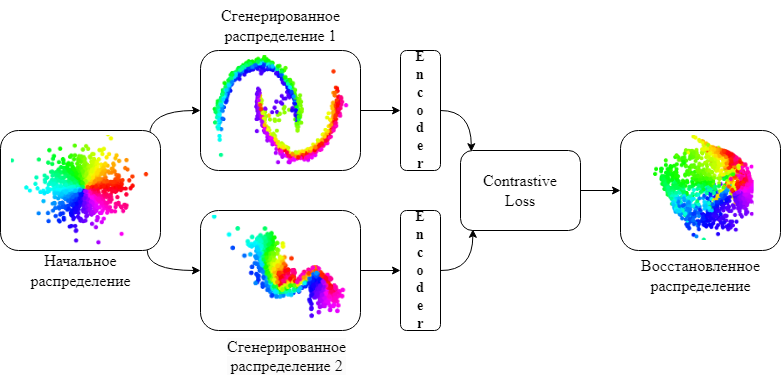
\includegraphics[scale = 0.65]{Pictures/Model.png}
    \caption{Схема модели искусственного эксперимента. Точки одинакового цвета получены из одной и той же точки начального распределения.}
    \label{fg:model}
\end{figure}

На рис.\ref{fg:model} представлена визуализация работы модели. Локальный минимум представленной функции потерь достаточно хорошо восстанавливает форму начального распределения. Также можно заметить артефакты, характерные для сгенерированных распределений. Например, более плотное скопление для точек красного и розового цвета и менее плотное -- для точек зелёного цвета. На практике не получится полностью смоделировать начальное распределение ввиду шумов и характерных особенностей для каждой модальности, однако приблизить к нему восстановленное распределение можно.

В качестве метрик качества приближения векторов в пространстве представления используется MAE и косинусное расстояние:

\[MAE = \frac{1}{n} \sum\limits_{i = 1}^n\|\mathbf{x}_i - \mathbf{y}_i\|.\]

\[Cosine = \frac{1}{n} \sum\limits_{i = 1}^n\frac{\langle \mathbf{x}_i, \mathbf{y}_i \rangle}{\|\mathbf{x}_i\| \cdot \|\mathbf{y}_i\|}.\]

\begin{table}[!ht]
\begin{center}
\caption{Метрики качества приближения векторов в пространстве представления для $\mathcal{L}_{N-pair}$ и $\mathcal{L}_{Pos}$}
\begin{tabular}{| c | c | c | c |}
\hline
& До модели & $\mathcal{L}_{N-pair}$ & $\mathcal{L}_{Pos}$ \\ \hline
MAE & 1.508 & 0.616 & \textbf{0.564} \\ \hline
Cosine & 0.080 & 0.897 & \textbf{0.911} \\ \hline
\end{tabular}
\label{res_classification}
\end{center}
\end{table}

\subsection{Классификация}
В первом вычислительном эксперименте проводится сравнение $\mathcal{L}_{N-pair}$ (\ref{eq:103}) и $\mathcal{L}_{\text{Pos}}^N(f)$ (\ref{eq:11}) в задаче классификации изображений. В качестве датасета используется CIFAR10 \citep{krizhevsky2009learning}, состоящий из 60000 цветных изображений размером 32x32 для классификации. Базовая модель: SimCLR \citep{chuang2020debiased} с энкодером ResNet18 \citep{he2015deep} и N-pair loss (\ref{eq:103}), оптимизатор -- Adam \citep{kingma2017adam}, шаг обучения 0.001, размер батча 256. Все модели тренируются 50 эпох и оцениваются линейным классификатором после получения эмбеддинга.

Сравнение результатов работы можно увидеть на рис.\ref{fg:acc} и в таблице \ref{res_classification}. В качестве метрики берётся топ-1 и топ-5 accuracy:

\[Acc_1 = \frac{TP + TN}{TP + FP + TN + FN}.\]

\[Acc_k = \frac{1}{n}\sum\limits_{i=1}^n[\mathbf{y}_i \in \hat{\mathbf{y}}_i^k].\]

\begin{figure}[!ht]
   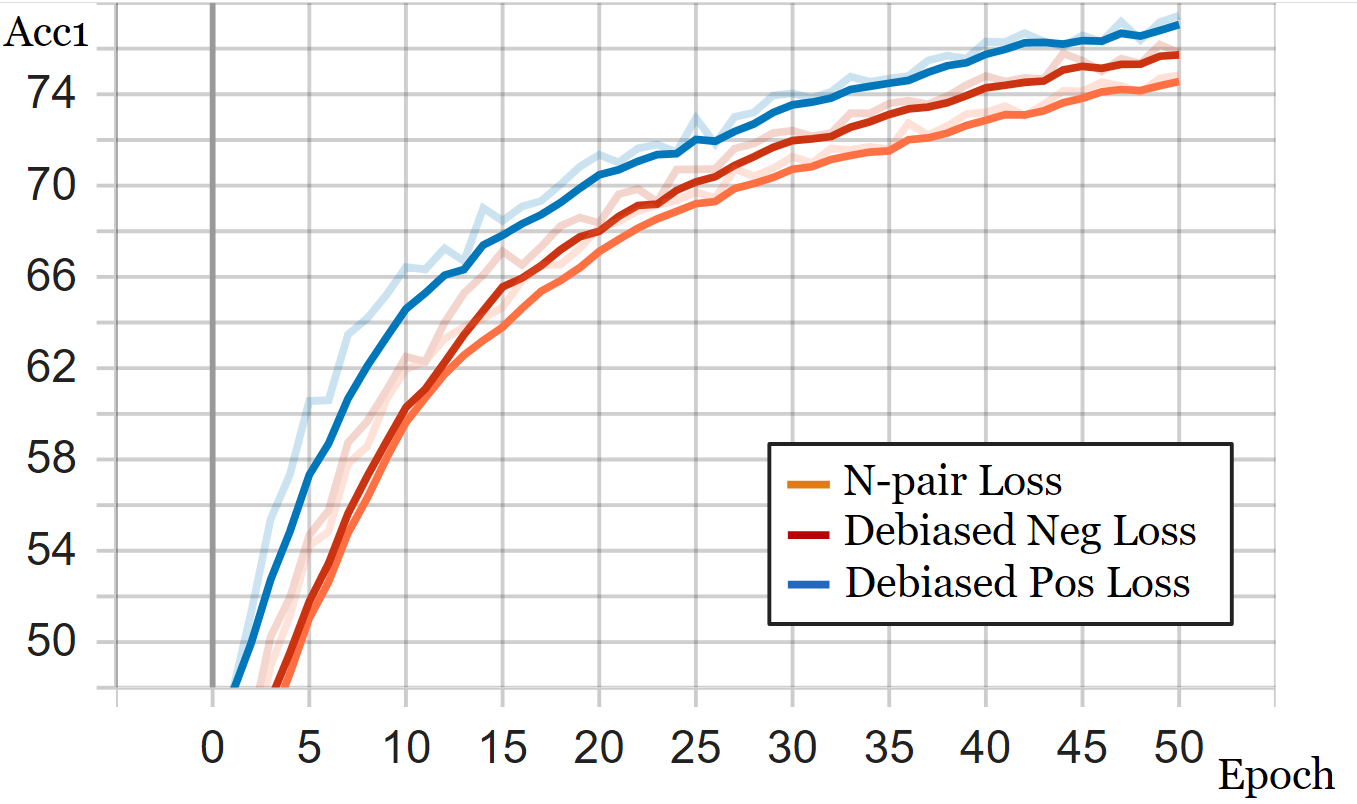
\includegraphics[width=0.5\textwidth]{Pictures/loss_acc1_new.png}
   \hfill
   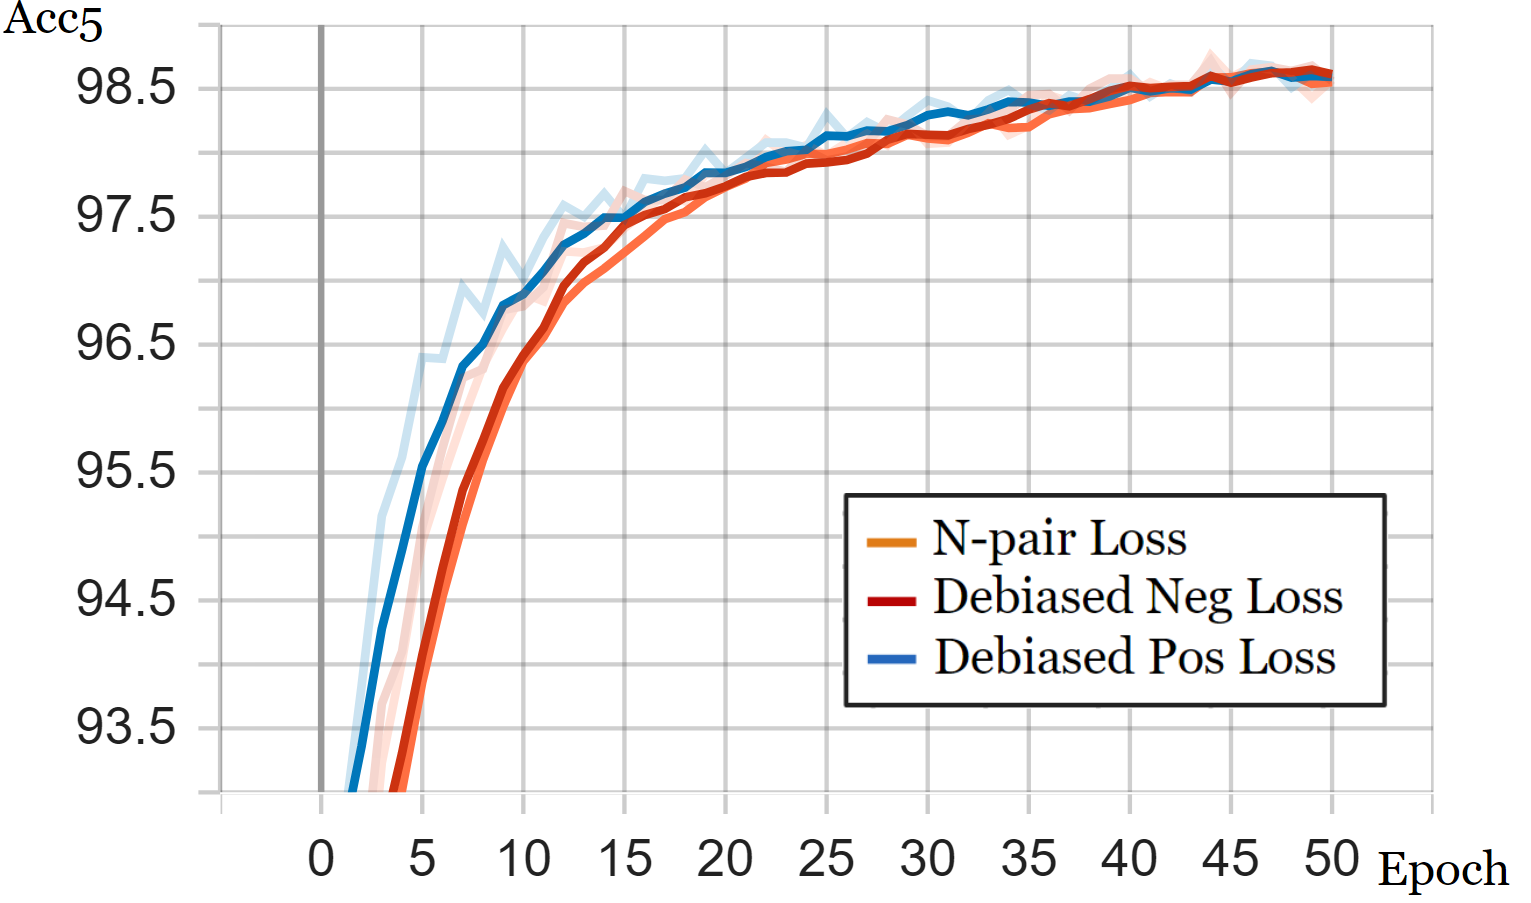
\includegraphics[width=0.5\textwidth]
   {Pictures/loss_acc5_new.png}
   \caption{Метрики acc1 и acc5 классификации с использованием N-pair loss, DebiasedNeg loss и DebiasedPos loss.}
   \label{fg:acc}
\end{figure}

\begin{figure}[!ht]
   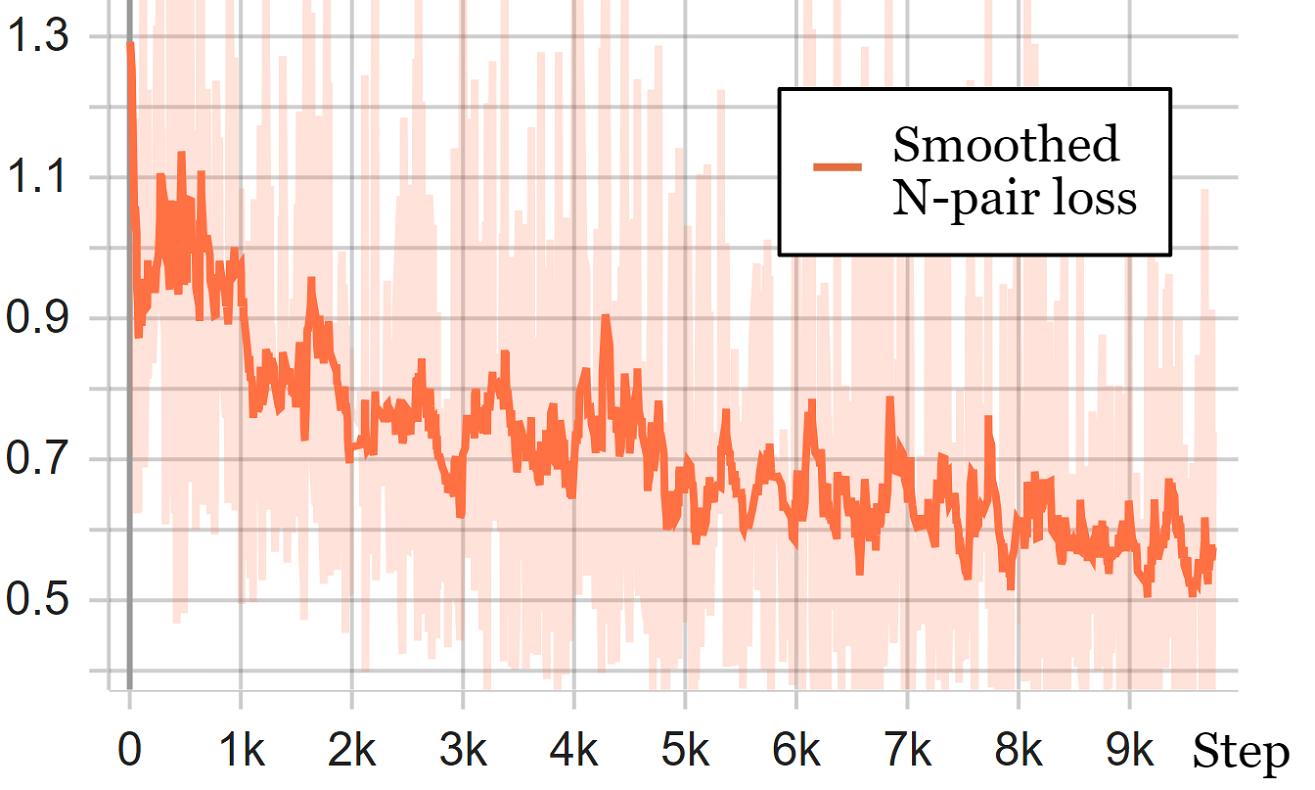
\includegraphics[width=0.5\textwidth]{Pictures/N-pair_loss.png}
   \hfill
   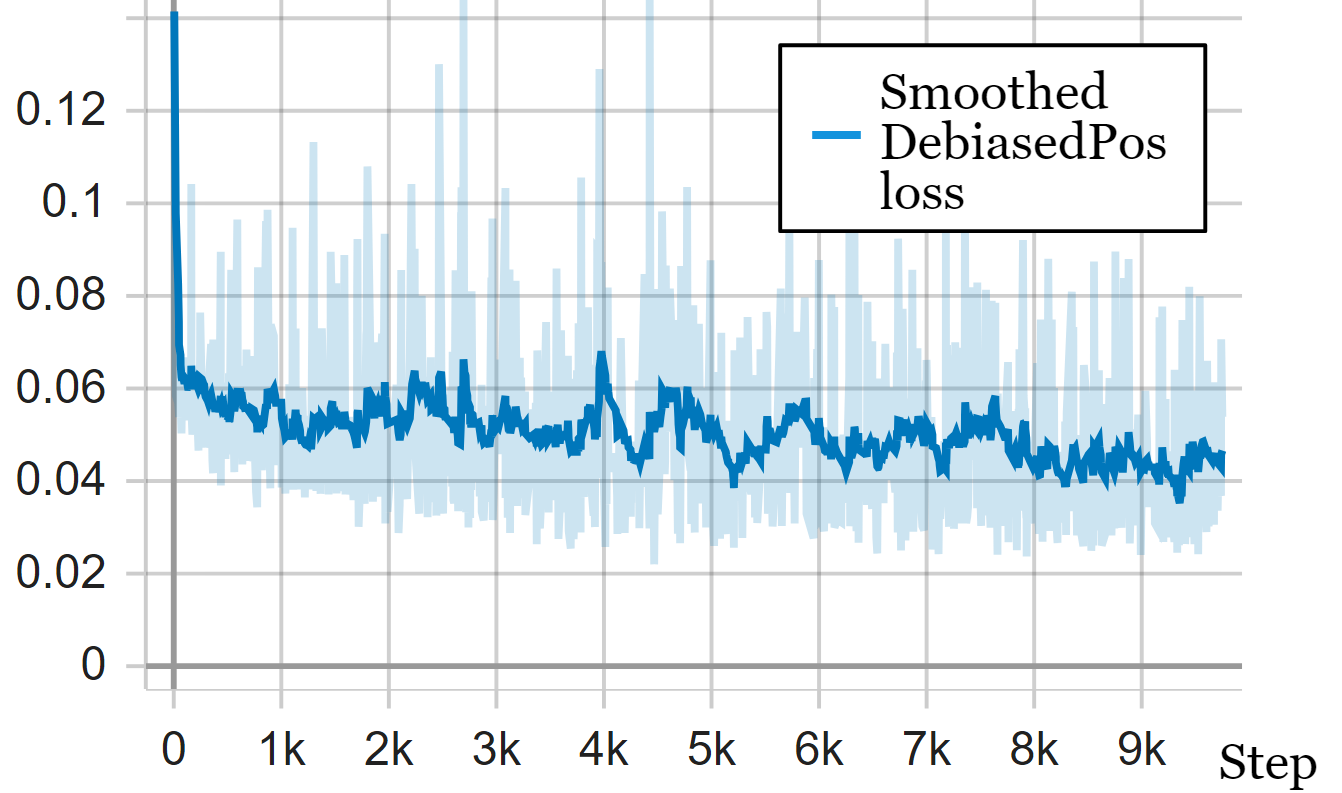
\includegraphics[width=0.5\textwidth]{Pictures/DebiasedPos_loss.png}
   \caption{Графики функции потерь для классификации с использованием N-pair loss и DebiasedPos loss.}
   \label{fg:acc}
\end{figure}

\begin{table}[!ht]
\begin{center}
\caption{Результаты классификации для $\mathcal{L}_{N-pair}$, $\mathcal{L}_{Neg}$ и $\mathcal{L}_{Pos}$}
\begin{tabular}{| c | c | c | c |}
\hline
& $\mathcal{L}_{N-pair}$ & $\mathcal{L}_{Neg}$ & $\mathcal{L}_{Pos}$ \\ \hline
Acc1 & 74.84 & 75.81 & \textbf{77.45}\\ \hline
Acc5 & 98.56 & 98.56 & \textbf{98.58}\\ \hline
\end{tabular}
\label{res_classification}
\end{center}
\end{table}

Модель, использующая $\mathcal{L}_{\text{Pos}}^N(f)$ имеет метрику топ-1 accuracy на $2.6\%$ лучше. Топ-5 accuracy по истечении 50 эпох у моделей одинаковая, однако для модели с $\mathcal{L}_{\text{Pos}}^N(f)$ метрика растёт быстрее.

\subsection{VQA}
В качестве большого эксперимента на реальных данных взята задача ответа на вопросы по изображению \citep{VQA}. Датасет состоит из 204 721 картинок из MS COCO \citep{lin2015microsoft}, 760 000 вопросов и около 10 миллионов ответов. Базовая модель -- TCL \citep{TCL} с функцией потерь $\mathcal{L} = \mathcal{L}_{cma} + \mathcal{L}_{imc} + \mathcal{L}_{lmi} + \mathcal{L}_{itm} + \mathcal{L}_{mlm}$, описанной выше. Визуальный энкодер представлен моделью ViT-B/16 с 12 слоями и 85.6M параметрами \citep{ViT}. Текстовый энкодер представлен первыми 6 и последними 6 слоями модели BERT$_{\text{base}}$ \citep{BERT} со 123.7M параметрами. Банк памяти содержит $K = 65536$ векторов, моментум $m = 0.995$. Оптимизатор -- AdamW \citep{AdamW}.

Все сравниваемые модели дообучаются с предложенной авторами \citep{TCL} предобученной модели при замороженном визуальном энкодере 5 эпох на 100 000 вопросах и оценивается на 50 000 вопросах. При аугментации из изображения вырезается часть размера $256 \times 256$. В качестве метрики используется accuracy, которая равна 1, если ответ модели находится в предложенном авторами VQA списке из 10 ответов для каждого вопроса.

Новые модели создаются посредством замены $\mathcal{L}_{N-pair}$ в $\mathcal{L}_{cma}$ (\ref{eq:cma}), $\mathcal{L}_{imc}$ (\ref{eq:imc}), $\mathcal{L}_{lmi}$ (\ref{eq:lmi}) на $\mathcal{L}_{Pos}$ и $\mathcal{L}_{Neg}$. В качестве метрики берётся число попаданий ответа модели в список из 10 ответов, предоставленных составителями датасета:

\[Acc = \frac{1}{n}\sum\limits_{i = 1}^n[\mathbf{y}_i \in \mathbf{y}_i^{10}].\]

Результаты представлены в таблице \ref{res_vqa}, пример работы моделей представлен на рис.\ref{fg:vqa}-\ref{fg:vqa_1}.

\begin{figure}[!ht]
    \begin{center}
    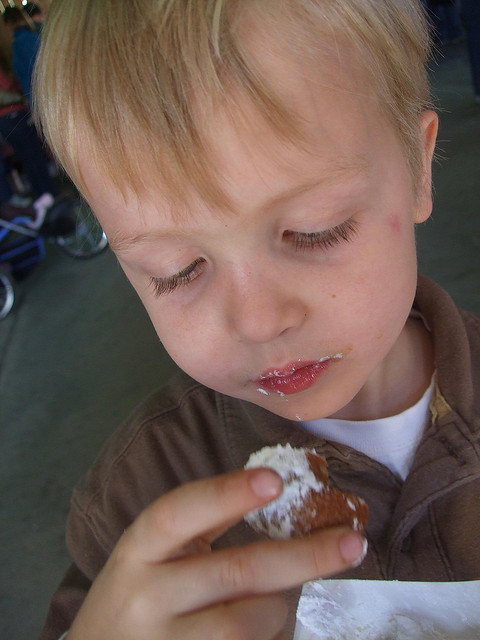
\includegraphics[scale = 0.4]{Pictures/contrastive_example.png}
    \caption{Пример работы модели в VQA-задаче. Вопрос: «What is the child eating?» Ответ модели с $\mathcal{L}_{N-pair}$ и с $\mathcal{L}_{Pos}$: «donut» входит в список верных.}
    \label{fg:vqa}
    \end{center}
\end{figure}

\begin{figure}[!ht]
    \begin{center}
    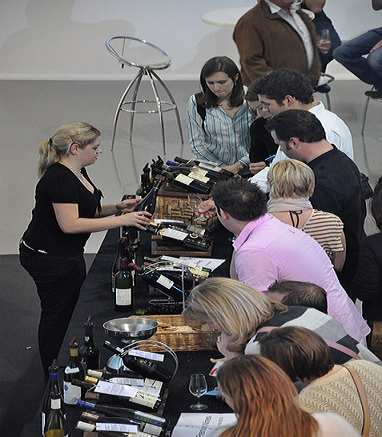
\includegraphics[scale = 0.85]{Pictures/image_3.png}
    \caption{Пример работы модели в VQA-задаче. Вопрос: «What kind of event are the people involved in?» Ответ модели с $\mathcal{L}_{N-pair}$: «party» неверный. Ответ модели с $\mathcal{L}_{Pos}$: «wine testing» входит в список верных.}
    \label{fg:vqa_1}
    \end{center}
\end{figure}

\begin{table}[!ht]
\begin{center}
\caption{Результаты VQA для $\mathcal{L}_{N-pair}$ и $\mathcal{L}_{Pos}$}
\begin{tabular}{| c | c | c |}
\hline
& $\mathcal{L}_{N-pair}$ & $\mathcal{L}_{Pos}$ \\ \hline
Accuracy & 66.29 & \textbf{67.23} \\ \hline
\end{tabular}
\label{res_vqa}
\end{center}
\end{table}

Пример на рис.\ref{fg:vqa_1} показывает, в каких случаях отсутствие учёта наличия смещения при плохой аугментации приводит к ошибке. Если при обучении для входа сети вырезается часть картинки без стола, то изображение перестаёт подходить под тематику дегустации. Тем самым генерируется неправильное представление и модель c $\mathcal{L}_{N-pair}$ даёт неверный ответ в отличие от модели с $\mathcal{L}_{Pos}$.

\newpage
\section{Заключение}
В данной работе проведён анализ смещения положительного и отрицательного распределения в задаче обучения сравнениями на примере эксперимента на искусственных двумерных данных, классификации изображений и мультимодальной задачи ответов на вопросы по изображениям. Предложена функция потерь, учитывающая шум при сэмплировании положительных элементов, доказана её сходимость к порождённому из кросс-энтропии $\mathcal{L}_{N-pair}$ и свойство максимизации совместной информации для положительной пары элементов выборки. В эксперименте на искусственных данных была рассмотрена способность предложенного метода при использовании регуляризации восстанавливать начальное распределение. В сравнении с $\mathcal{L}_{N-pair}$ и $\mathcal{L}_{Neg}$ предложенная функция потерь показала лучший результат в задаче классификации и в задаче ответов на вопросы.

\newpage
\bibliographystyle{plain}
\bibliography{references.bib}

\end{document}
